\section{Principio de funcionamiento entorno matlab y aspectos relacionados con las ecuaciones} 
\subsection{modelo del circuito empleado}

\begin{figure}[ht!]
    \centering
    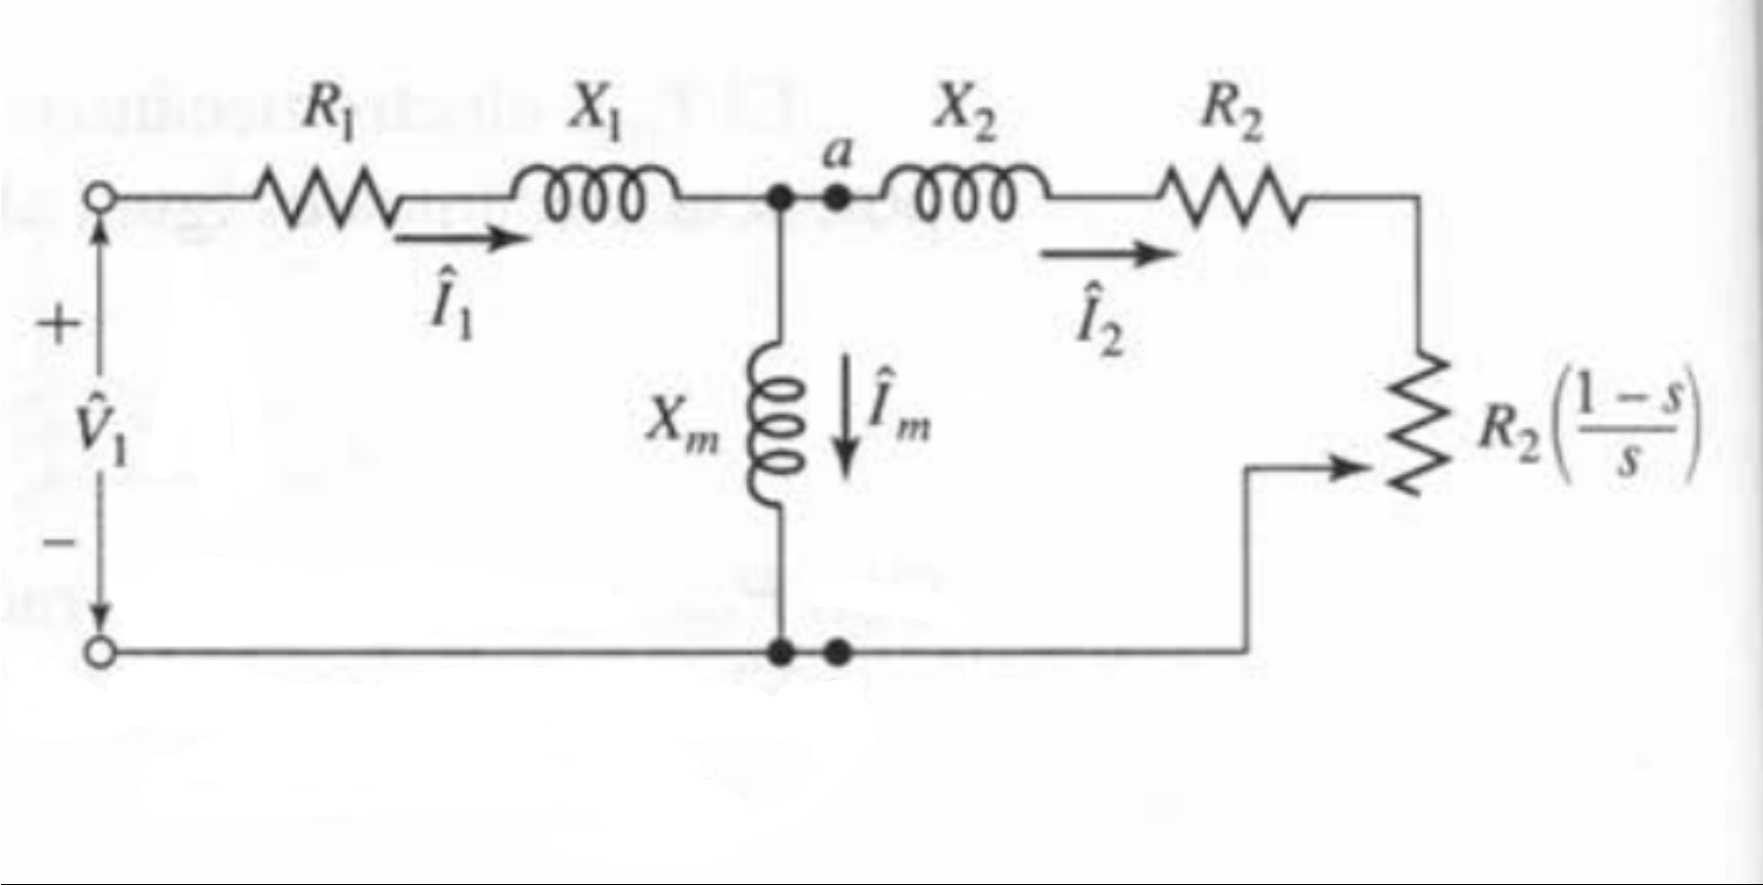
\includegraphics[width=0.48\textwidth]{imginterfaz/circuito equivalente.png}
    \caption{Modelo del circuito equivalente del motor de inducción.}
    \label{fig:circuitoEquivalente}
\end{figure}

\subsection{Aspectos inciales con el desarrollo de la interfaz}
Si bien para el entorno matlab App Designer es un poco tedioso al principio de entender se parte de identificar las entradas y salidas.

\begin{figure}[ht!]
    \centering
    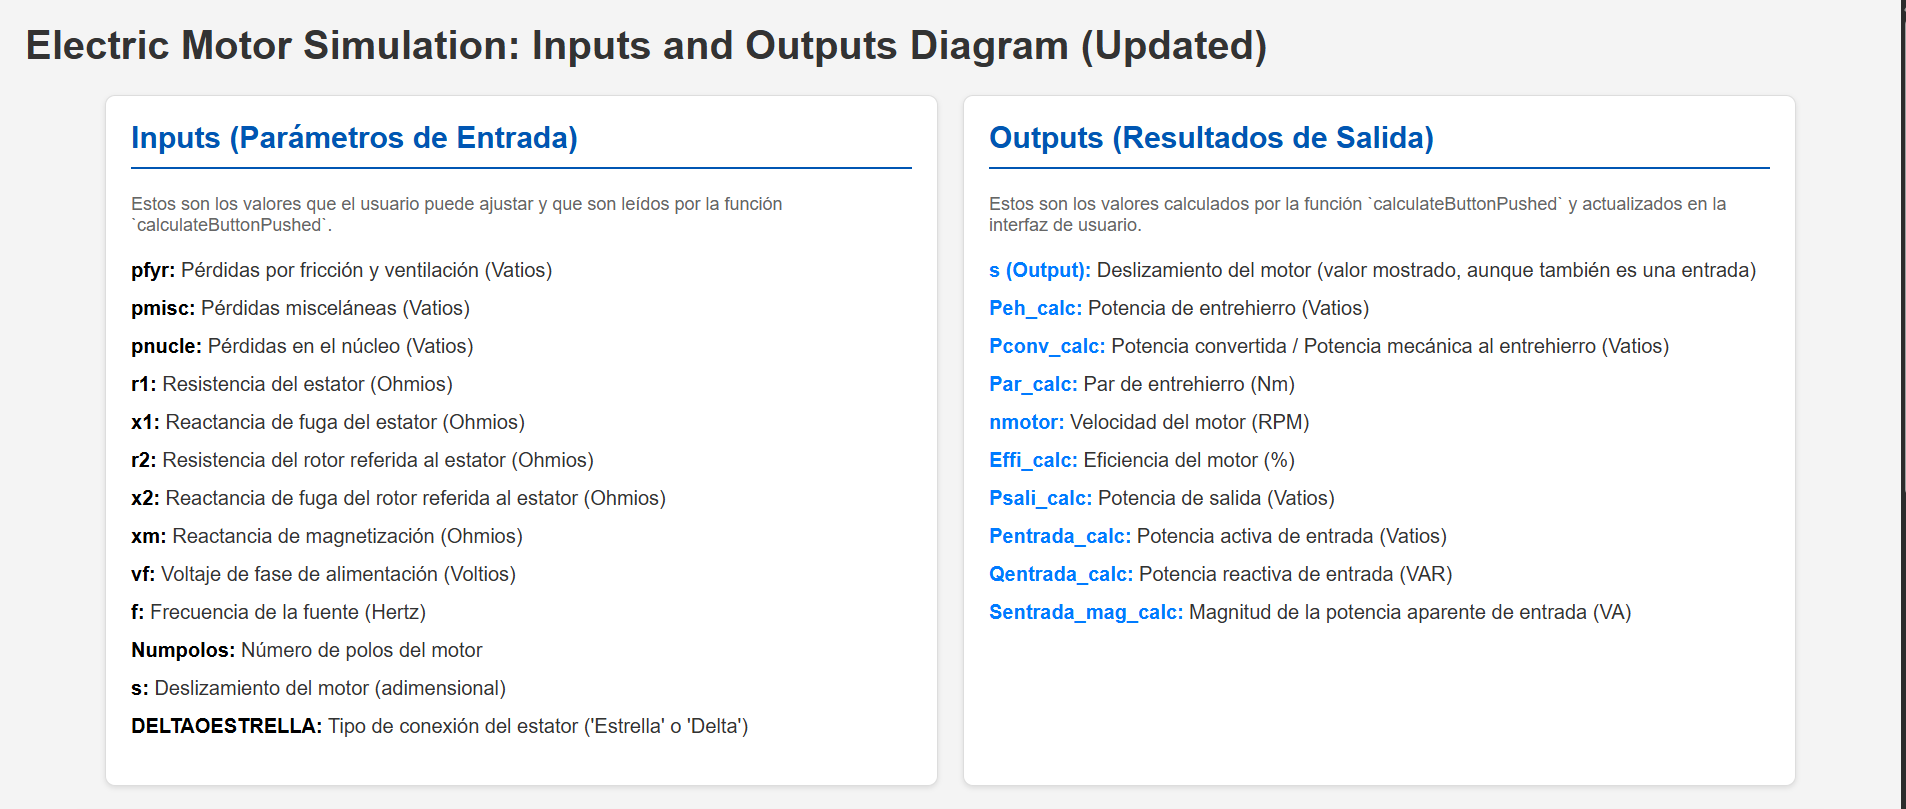
\includegraphics[width=0.48\textwidth]{imginterfaz/identificandoEntradas.png}
    \caption{Entradas y Salidas.\label{fig:identificandoEntradas}}
\end{figure}
En la figura \ref*{fig:identificandoEntradas} se menciona calculateButtonPushed, dicho botón que iniciará el funcionamiento de la interfaz.




\begin{figure}[ht!]
    \centering
    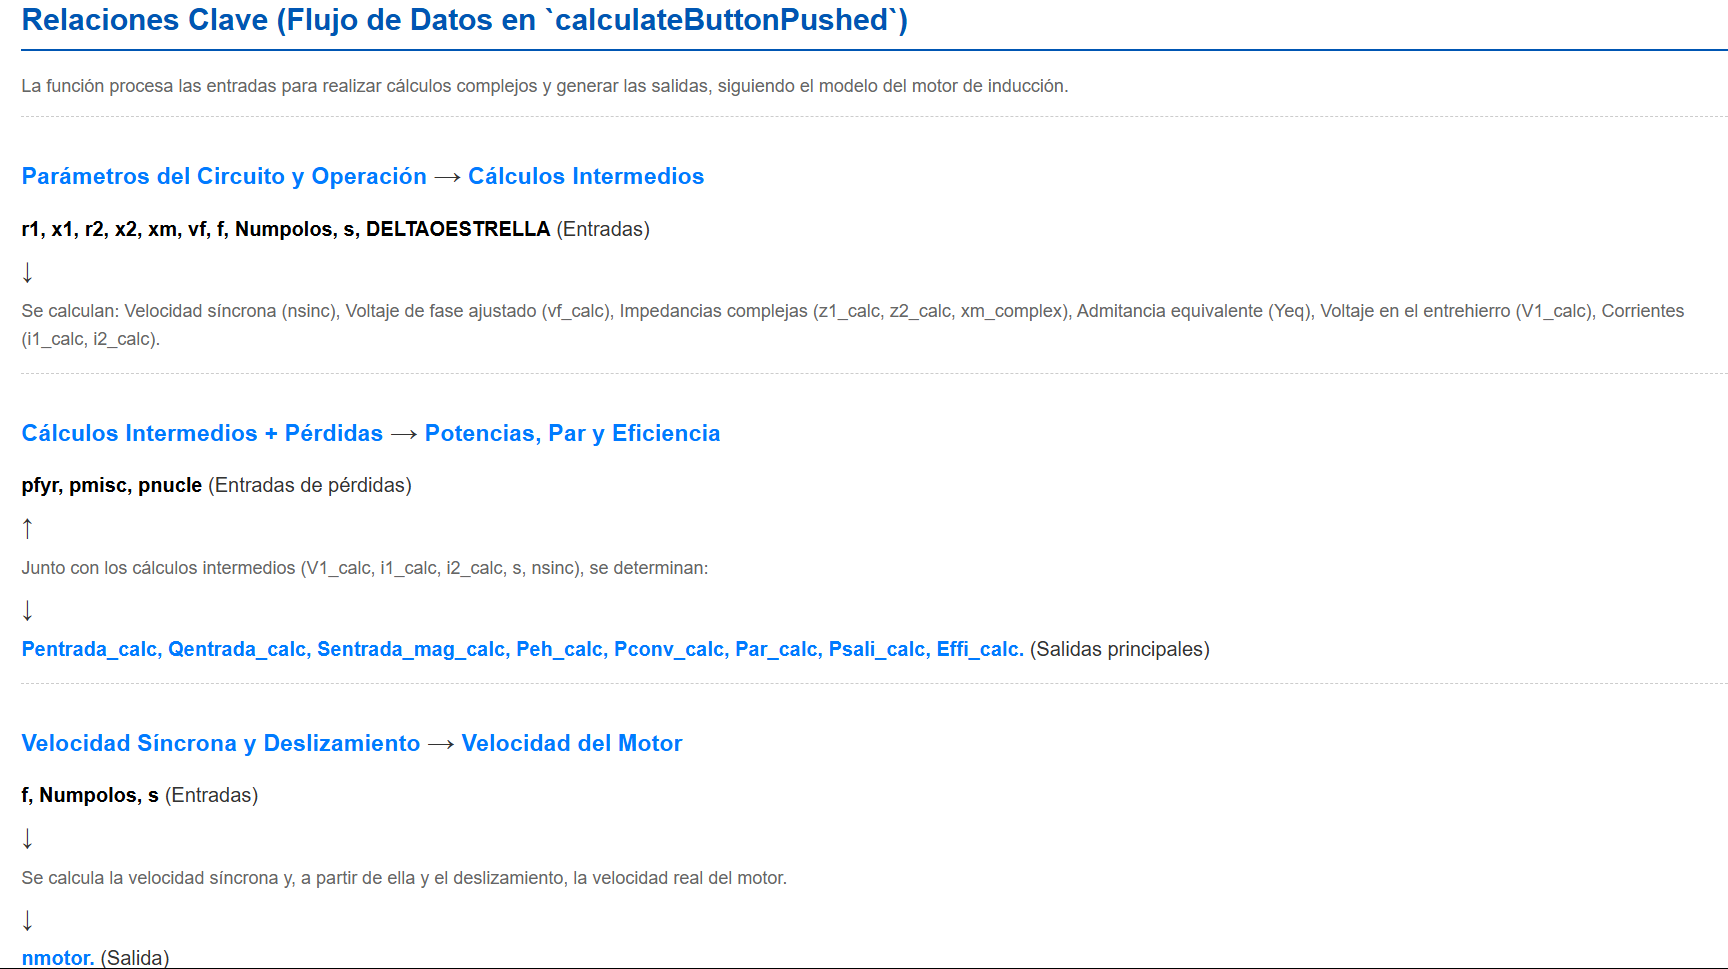
\includegraphics[width=0.48\textwidth]{imginterfaz/button.png}
    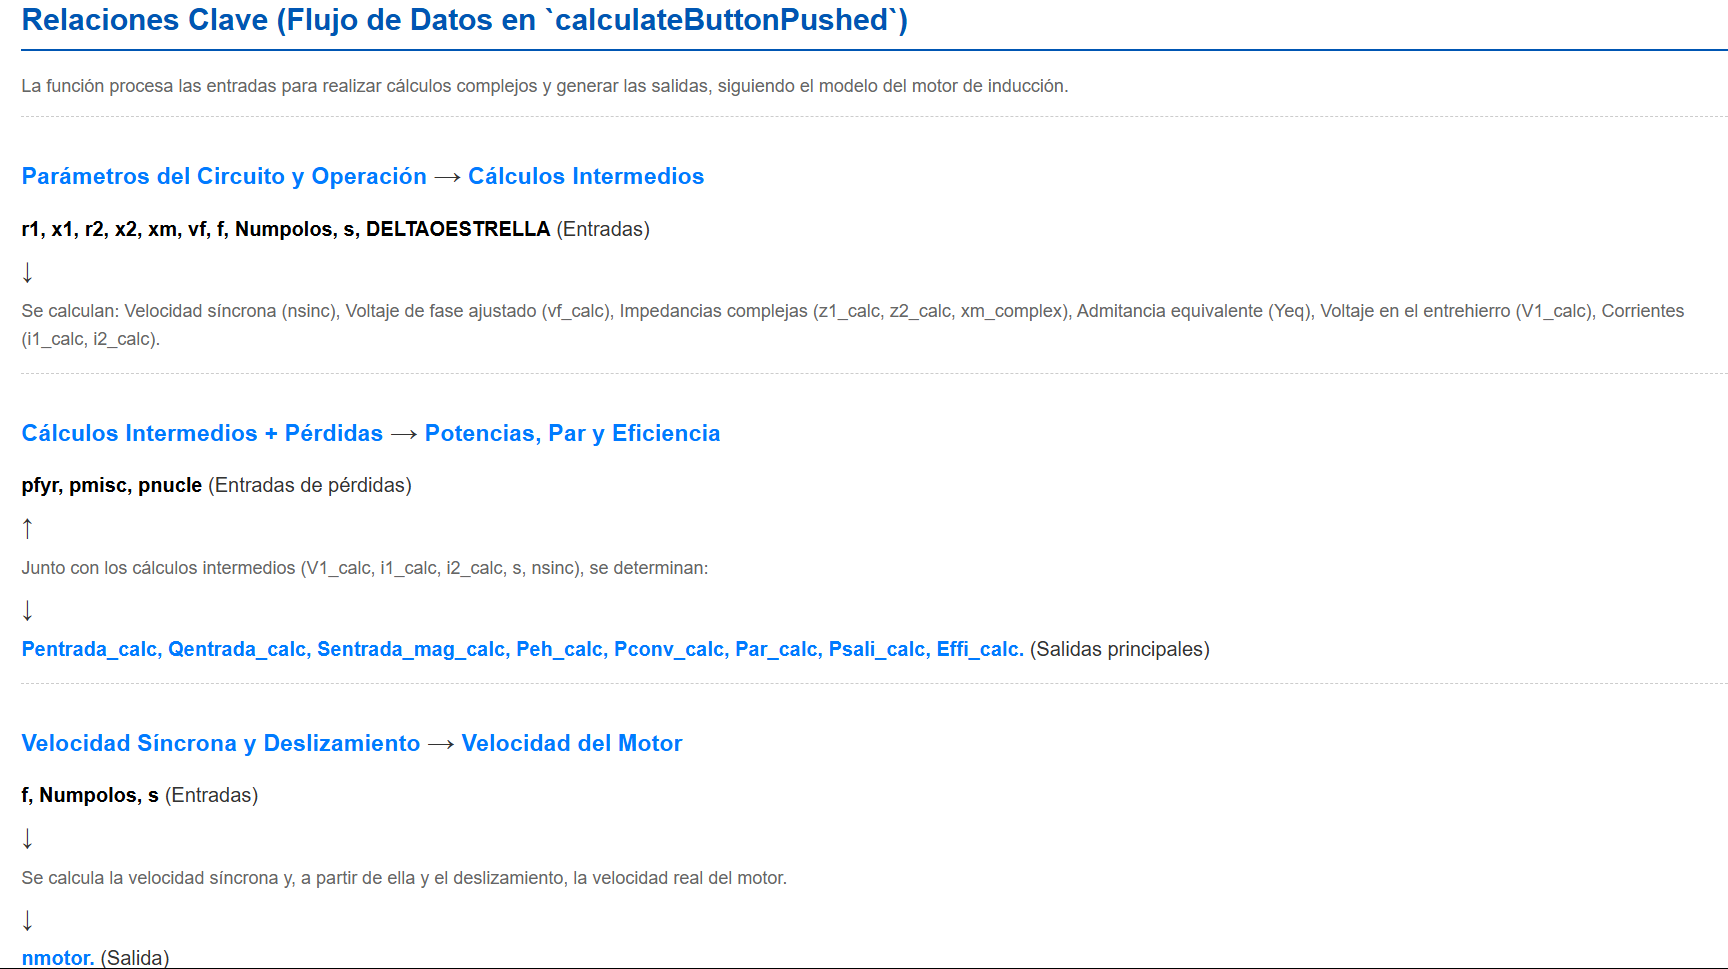
\includegraphics[width=0.48\textwidth]{imginterfaz/button.png}
    \caption{Flujo de datos de las entradas para obetener las salidas.\label{fig:button}}
\end{figure}

De la figura \ref*{fig:button} se puede observar que el flujo de datos de manera muy simplificada es el siguiente:
\begin{itemize}
    \item Se ingresan los valores de las entradas.
    \item Se presiona el botón de calcular.
    \item Se ejecuta la función que calcula los valores de salida.
    \item Se muestran los resultados en la interfaz.
    \item Se grafican los resultados.
\end{itemize}


\subsection{Aspectos relacionados con la intefaz}
En la construccion de la interfaz primero se partio del diseño de la misma, teniendo en cuenta los parametros ademas de elementos como 2 sliders y editores de texto numericos tanto para las variables de entrada como de salida.
   



Finalmente se puede observar el diseño de la interfaz con las entradas y salidas con sus respectivas unidades.
\begin{figure}[ht!]
    \centering
    \includegraphics[width=0.48\textwidth]{imginterfaz/interfaz.png}
    \caption{Interfaz de usuario.}
    \label{fig:interfaz}
\end{figure}